%%%%%%%%%%%%%%%%%%%%%%%%%%%%%%%%%%%%%%%%%%%%%%%%%%%%%%%%%%%%%%%%%%%%%%%%%%%%%%%%
 Fruit such as apples, grapes, blueberries, etc grows in clusters of arbitrary size and shape. While for some of them it is good enough to extract the volume of a cluster (e.g., grapes) for others (e.g., apples) it is essential to compute the exact fruit counts for accurate yield mapping. Methods that only detect fruit fail to offer general solutions to estimate accurate fruit counts and overall yield. Therefore, it is essential to have a fruit counting module following detection.
 
 Counting clustered fruit from a running sequence of images is difficult for three main reasons. First, there is a trade-off between image footprint and the size of individual fruit in the image. If we use close-up views, coverage becomes tedious. On the other hand, if we use a wide-angle camera,  individual fruit occupies only a small area in images. Second, fruit can be found in arbitrarily shaped clusters in which almost all fruit overlap with each other. Segmenting individual fruit from such cluster images is challenging. Third, because of occlusions due to leaves and branches as well as specularities sometimes fruit is not detectable at all. 

Many yield estimation systems do not focus on accurate counting. Instead, these systems rely on developing a consistent estimator of actual fruit count. These methods include Wang et. al~\cite{wang} who used morphological operations and ellipse fitting for counting. Their method does not handle more than two fruit in a cluster. Hung et. al~\cite{hung2015feature} relied on circular Hough transformation to extract individual fruit. Linker et. al~\cite{Linker}  presented a method based on fruit edge detection. This method requires very high-resolution images. All these techniques work for simple instances such as those shown in  Fig.~\ref{fig:sapple1}. In more challenging, yet common instances (see Fig.~\ref{fig:capple1}), both Hough transform and ellipse fitting will fail. 

In recent times, many researchers used state-of-the-art object detection network Faster R-CNN (FRCNN) to solve fruit detection and counting in a combined way~\cite{bargoti_deep_2017,sa_deepfruits:_2016}. These approaches fail when one fruit is heavily occluded by others, as seen in Fig. ~\ref{fig:main2a}. In this case, the network generates $2000$ region proposals for image patches of $500 \times 500$ pixels, which are moved over the image with stride $50$ pixels. All the proposals are then merged and filtered using Non-maximum suppression (NMS) with an Intersection over Union (IoU) threshold of $0.7$. Owing to the wrong NMS threshold, the method misses one of the apples in the cluster (Fig. ~\ref{fig:main2b}). Bargoti and Underwood~\cite{bargoti_deep_2017} found that their approach contains errors of ∼ $4\%$ due to the NMS threshold.

Therefore, to identify the number of fruit correctly and to locate individual fruit from these images we need novel models and techniques. In this chapter, we present two such methods: one for counting the fruit based on a classic unsupervised clustering technique- Gaussian Mixture Models(GMM)~\cite{em} and another using an intuitive greedy circle fitting algorithm. The clustering technique is robust and accurate. The greedy method is identical to the state of the art techniques such as circular Hough transform and ellipse fitting. We use it as a baseline for comparison with the performance of the GMM method. Besides, we provide comparisons with a deep learning approach~\cite{hani_apple_2018,hani_jfr_counting} that can compute the fruit counts without the detection masks. We start with our technical approach in the next section.

\begin{figure}[tbp]
        \centering
        \begin{subfigure}[b]{.3\textwidth}
        \centering
            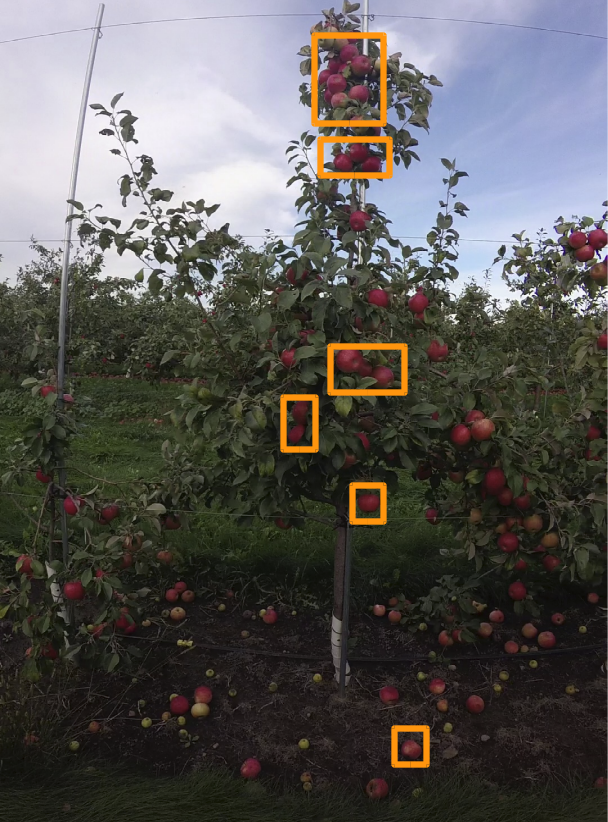
\includegraphics[width = \textwidth]{figures/counting/original}           
         \caption{Original Image}
         \label{fig:singorig}
       \end{subfigure}\quad \begin{subfigure}[b]{.3\textwidth}
       %\centering
       \begin{subfigure}[b]{\textwidth}
       %\centering
            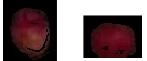
\includegraphics[width = \textwidth]{figures/counting/sapple1}           
         \caption{Single Apples}
         \label{fig:sapple1}
         \end{subfigure}
         \begin{subfigure}[b]{\textwidth}
        % \centering
            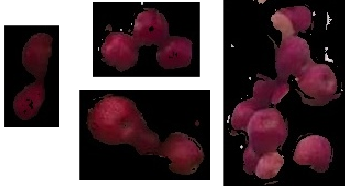
\includegraphics[width = \textwidth]{figures/counting/capple1}           
         \caption{Apple Clusters}
         \label{fig:capple1}
         \end{subfigure}
       \end{subfigure} \quad \begin{subfigure}[b]{.3\textwidth}
              
       \begin{subfigure}[b]{\textwidth}
       \centering
            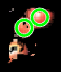
\includegraphics[scale = .8]{figures/counting/simplegreedy1}
         \caption{Detected apples by the greedy method}
         \label{fig:greedy}
       \end{subfigure}
       \begin{subfigure}[b]{\textwidth}
       \centering
            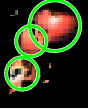
\includegraphics[scale = .5]{figures/counting/gmmcomp}
         \caption{Detected apples by GMM method}
         \label{fig:gmcomp}
       \end{subfigure}
       \end{subfigure} 
   \caption[Fruit counting in apple orchards.]{A sample image and few example apple clusters. Fig. (\subref{fig:sapple1}) shows two example single apples. These apples can be detected easily by state of the art methods such as circular Hough transform or ellipse fitting. It is hard to generalize these methods for more complex clusters shown in fig.(\subref{fig:capple1}). Fig. (\subref{fig:greedy}) shows a sample output from the greedy circle fitting method. Fig. (\subref{fig:gmcomp}) shows the output of GMM method on the same input.}
   \label{fig:groupex}
\end{figure}    


 %It is unable to detect the partially visible apple
 
%It successfully finds the apple missed by a greedy method
\begin{figure}[b]
    \centering
    \begin{subfigure}[b]{.45\textwidth}
    \centering
    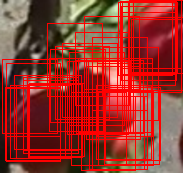
\includegraphics[width=0.45\columnwidth]{figures/counting/detectionProblem1}
    \caption{Output of Faster R-CNN}\label{fig:main2a}%
    \end{subfigure}    \quad\begin{subfigure}[b]{.45\textwidth}
    \centering
    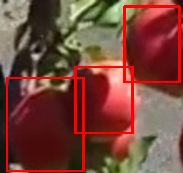
\includegraphics[width=0.45\columnwidth]{figures/counting/detectionProblem2.pdf}
    \caption{Output after thresholding and NMS }\label{fig:main2b}%
    \end{subfigure}
    \caption[Counting with Faster R-CNN]{Case of undercounting of Faster R-CNN}
    \label{fig:failureRCNN}
\end{figure}


%%%%%%%%%%%%%%%%%%%%%%%%%%%%%%%%%%%%%%%%%%%%%%%%%%%%%%%%%%%%%%%%%%%%%%%%%%%%%%%%
\section{Technical Approach}\label{sec:technical}
%$I_1, I_2, ...,I_n$
%$I$
Given a set of segmented input images, we want to find the number and location of all the fruit in every image. In this section, we propose two different methods for solving this problem: first using Gaussian Mixture Models (GMM) and second based on greedy circle fitting. The greedy circle fitting approach provides a baseline for comparison. As the first step for both methods, we perform a connected component analysis on the input image and detect all the individual clusters. We compute the location and radius of each fruit in each cluster. As the clusters are disjoint the total number of fruit can be obtained by simply summing up the numbers across all clusters.



\subsection{Unsupervised Clustering Using Gaussian Mixture Model} \label{subsec:gmmcount}
Given a segmented input image, we would like to find the number and location of all the fruit in the image. We use a Gaussian Mixture Models (GMM) based clustering method. Instead of color, we now focus on the spatial components of the image. This method holds numerous advantages over the Circular Hough Transform (CHT) based techniques (\cite{cht}) - it does not require manual parameter tuning, can handle a significant level of occlusion and find fruit of rapidly varying size.

In our method, each fruit is modeled by a Gaussian probability distribution function (pdf) and fruit clusters are modeled as a mixture of Gaussians. We start by converting the input cluster image $I$ to binary. Let this binary image be denoted by $I_{b}$. The locations of the non-zero pixels in the binary image are used as input to GMM. 

%\subsubsection{Model:\\}
\noindent Let X represent the set of fruit we are trying to find. Then, we can convert our problem to a Gaussian mixture model formulation in the following way:
\begin{equation}
P(I_b|X) = G^k(\phi,\mu,\Sigma) = \sum_{i = 1}^k \phi_{i} G_{i}(\mu_{i},\Sigma_{i})
\end{equation}

Here, $G^k(\phi,\mu,\Sigma)$ is a Gaussian mixture model with  $k$ components, and $G_{i}$ is the $i$~th component of the mixture. $\mu_{i}$ and $\Sigma_{i}$ are the mean and covariance of the $i^{th}$ component. The covariance matrix $\Sigma_{i} = \left[\sigma_{x_{i}}^2,\sigma_{y_{i}}^2\right]$ is diagonal. $\phi_{i}$ is the weight of the $i^{th}$ component where $\sum_{i= 1}^k \phi_{i} = 1$ and $0\leq \phi_{i}\leq 1$. 

Given model parameters $\theta = \{ \phi, \mu, \Sigma \}$, 
the problem of finding the location of the center of the fruit and their pixel diameters can be formulated as computing the world model which maximizes $P(I_b|X)$.

Each component $G_{i}(\mu_{i},\Sigma_{i})$ of the mixture model represents an fruit with center at $\mu_{i}$, equatorial radius $2\sigma_{x_{i}}$ and axial radius $2\sigma_{y_{i}}$. 


\noindent A common technique to solve for $\arg \max P(I_b|X)$ is the expectation-maximization (EM) algorithm (\cite{em}). As is well-known, EM provides us a local greedy solution to the problem. Since EM is susceptible to local maxima, initialization is very important. We used K-means++ (\cite{kmeans}) (which uses randomly-selected seeds to avoid local maxima) for initialization of EM. 

\textbf{Selecting the Number of Components:} In our problem formulation, the number of components $k$ is the total number of fruit in image $I$. EM enables us to find the optimal location of the fruit given the total number of fruit $k$. Our main technical contribution is a method to calculate the correct $k$. Let the correct number of fruit in the input image be $\kappa$. We tried different state-of-the-art techniques (Akaike Information Criterion (AIC) (\cite{mdt}), Minimum Description Length (MDL) (\cite{mdt}) etc.) for finding $\kappa$. None of them worked out of the box for our purposes (Fig.~\ref{fig:aic}). Therefore, we propose a new heuristic for evaluating mixture models with a different number of components based on MDL. 

\begin{figure}[!hbpt]

        \centering        
            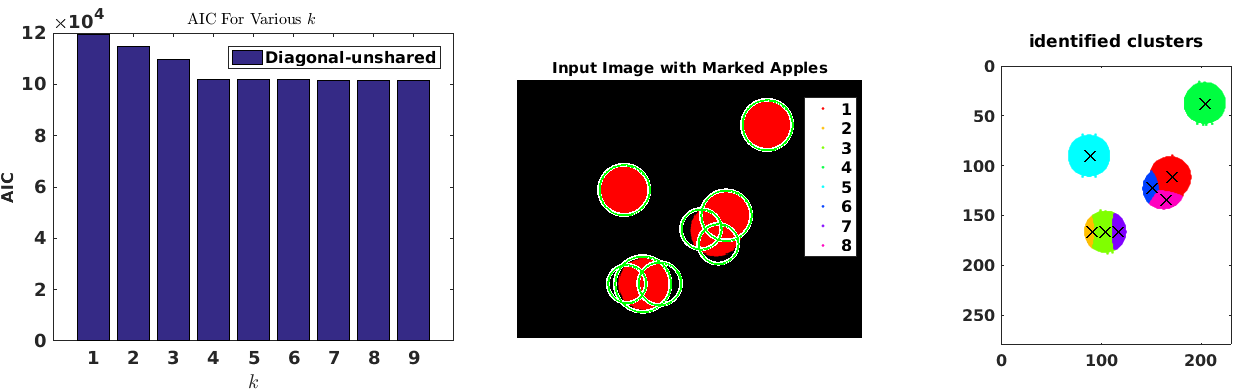
\includegraphics[width=\textwidth]{figures/counting/AIC.png}           
        
   \caption[Failure of popular model section criteria.]{Popular methods like AIC/BIC do not work out of the box for our purposes. These criteria tend to choose higher values of $k$. In this synthetic image, we have only five circles but the AIC based criterion value (Bar plot in the middle) was lowest for $k = 6$ and consequently, it finds eight fruit.}
   \label{fig:aic}   
\end{figure}    



Let  $\sigma_{min} = min(\sigma_{x_{i}},\sigma_{y_{i}})$ and $\sigma_{max} = max(\sigma_{x_{i}},\sigma_{y_{i}})$. Using the mean and covariances of the $i$th component we define a $2D$ Gaussian kernel $\mathcal{G}(\mu_{i},\sigma_{max})$ where  $\sigma_{max}$ is the variance. Let $P(\mu_{i})$ denote the response of the kernel when placed at the center $\mu_{i}$ in the original input image $I$ and $C_{i}$ denote the total number of pixels clustered by $G_{i}(\mu_i,\Sigma_i)$. For each component $G_{i}(\mu_i,\Sigma_i)$, of the mixture model $G^k(\phi,\mu,\Sigma)$ we define the reward $R_{i}$ in the following way,

\begin{equation}
\begin{split}
R_i(G_{i}) =  \phi_{i}\left[ P(\mu_{i})+  P(\mu_{i})\left(\frac{\sigma_{min}}{\sigma_{max}}\right)^2 +\right. \\ \left.  P(\mu_{i})\frac{C_{i}}{\pi \sigma_{max}\sigma_{min}} - \frac{1}{3}\left( \pi\sigma_{x_{i}}\sigma_{y_{i}} -C_{i} \right) \right]
\end{split}
\label{eq:reward}
\end{equation}

For most of the images, we only capture the frontal views of the fruit, which can be easily approximated by circles lying on a plane. All four terms in equation~\eqref{eq:reward} reward specific spatial characteristics of the Gaussian pdf related to this fact. $P(\mu_{i})$ represents the strength of the distribution in terms of pixel values and is present in the first three terms. The second term rewards circular-shaped distributions using the eccentricity of the pdf. As the eccentricity $\epsilon = \sqrt{1- \frac{\sigma_{min}^2}{\sigma_{max}^2}}$ for circles is zero, we use $1-\epsilon^2 = \left(\frac{\sigma_{min}}{\sigma_{max}}\right)^2$ as the rewarding factor. The third term rewards coverage. The fourth term penalizes Gaussian pdf covering large areas and clustering very few points.

Now if we find out the reward $R_i(G_{i}(\mu_i,\Sigma_i))$ for all the components $k$, the total reward for the mixture model $G^k(\phi,\mu,\Sigma)$ can be computed by summing them together.



Next, we define the penalty term. The traditional MDL penalty term is $U = c p \log(|Y|)$ where $p$ is the number of parameters in the model, $|Y|$ is the total size of the input data, and $c = \frac{1}{2}$ is a constant. Based on this principle, our penalty term is  $V(G^k(\phi,\mu,\Sigma))$ is defined as the following
\begin{equation}
V(G^k(\phi,\mu,\Sigma)) = c'(3k) \log(\sum_{\vec{x}}(I_b(\vec{x}) \neq 0)))
\label{eq:penalty}
\end{equation}
where $x$ represents the pixel index across the image $I_b$. Compared to the traditional MDL based penalty we have the constant $c' =\frac{3}{2}$ instead of $c =\frac{1}{2}$. This is attributed to the fact that the reward expression~\eqref{eq:reward} has three terms compared to one. The number of components $k$ is multiplied by three as each Gaussian has three parameters $\left[\mu_i,\sigma_{x_i}, \sigma_{y_i}\right]$. With these terms defined, we choose the correct number of components $\kappa$ in the following way:

\begin{equation}
\kappa = \argmax{k} R(G^k(\phi,\mu,\Sigma))- V(G^k(\phi,\mu,\Sigma))
\label{eq:numcomp}
\end{equation}

\begin{figure}[!hbpt]
\begin{subfigure}{\textwidth}
        \centering        
            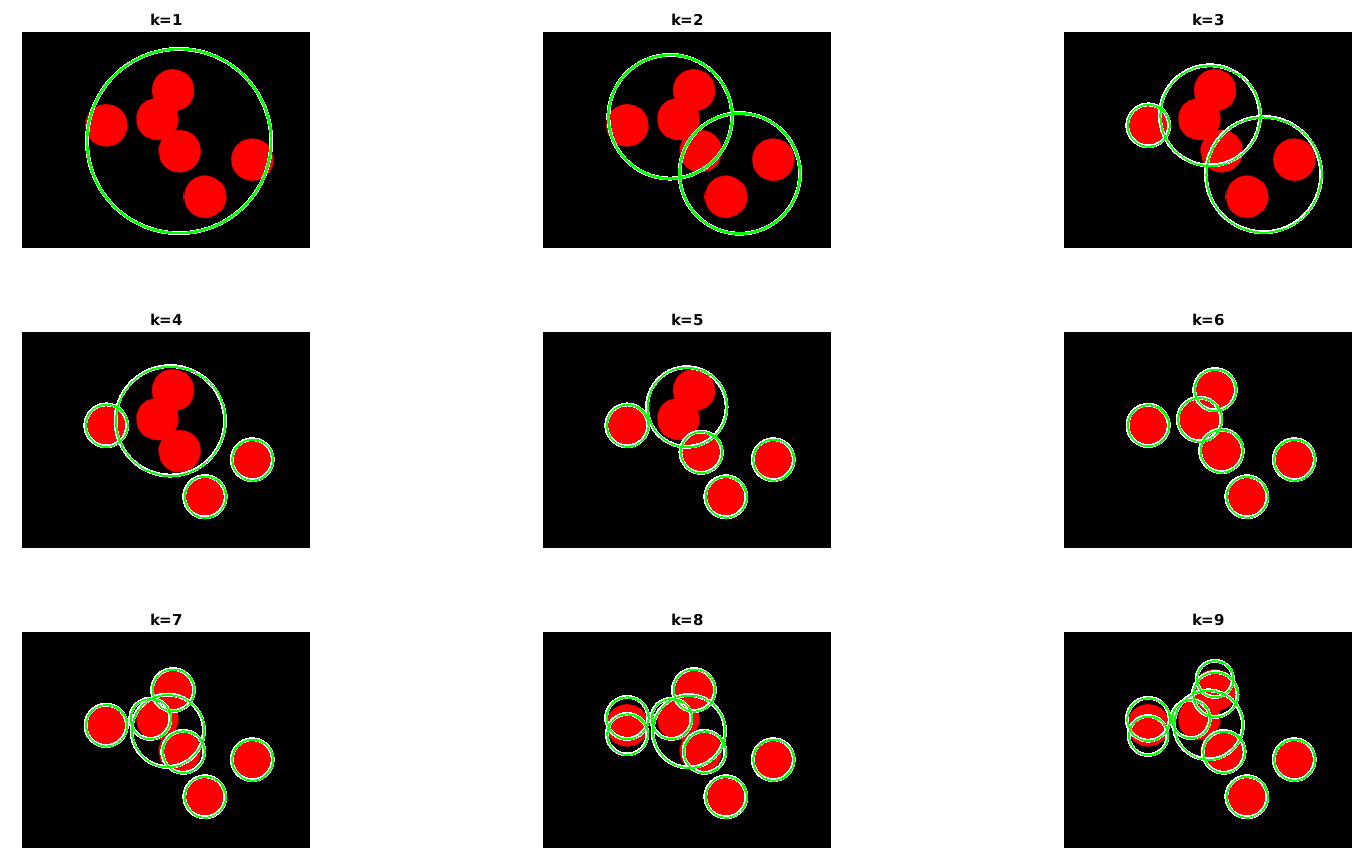
\includegraphics[width = \textwidth]{figures/counting/isersyncov.png}           
        
   \caption{Predicted circles for different number of components in GMM.}
   \label{fig:gmmsyn}
   \end{subfigure}\\ \begin{subfigure}{\textwidth}
   \centering
   \begin{subfigure}{.32\textwidth}
   \centering
            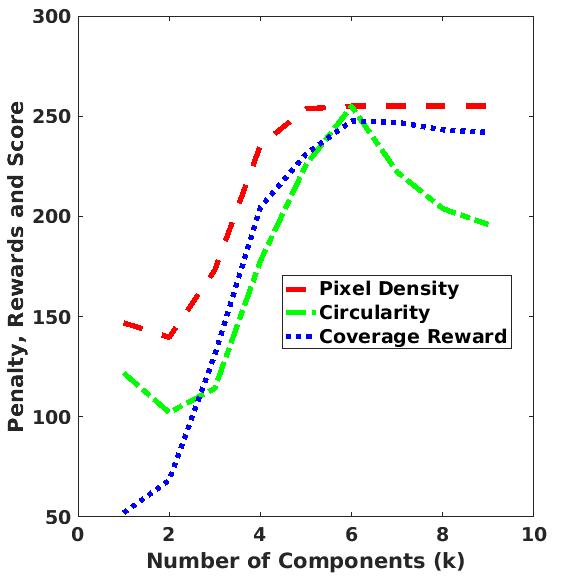
\includegraphics[width = \textwidth]{figures/counting/iserscorepart11.png} 
            \caption{Rewards.}
        \label{fig:gmmkplotrew}               
       \end{subfigure}\begin{subfigure}{.32\textwidth}  
       \centering
       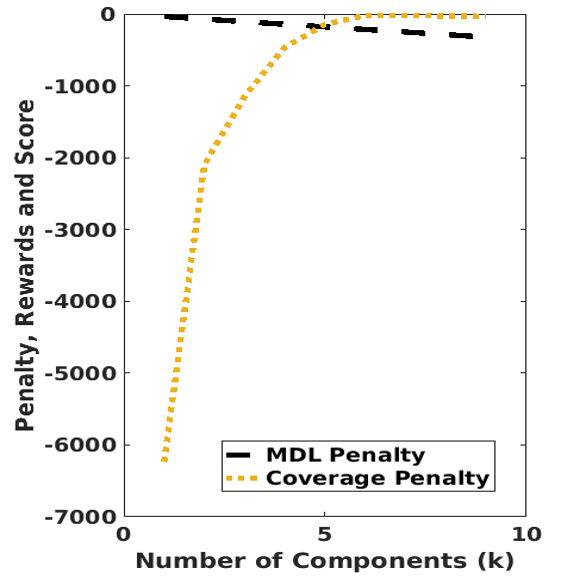
\includegraphics[width = \textwidth]{figures/counting/iserscorepart22.png} 
            \caption{Penalties.}
        \label{fig:gmmkplotpen}    
       \end{subfigure} \begin{subfigure}{.32\textwidth}   
       \centering
       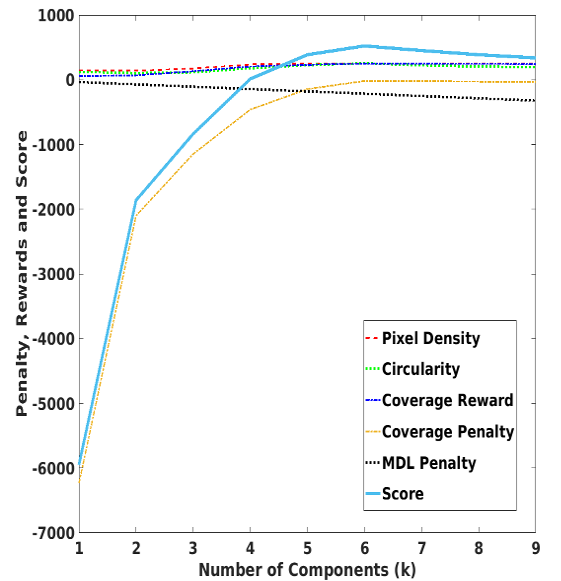
\includegraphics[width = \textwidth]{figures/counting/iserscorepart33.png} 
            \caption{Final score.}
        \label{fig:gmmkplot}   
       \end{subfigure}
       \end{subfigure}
  \caption[Fruit counting on synthetic data using unsupervised clustering.]{A synthetic example consisting of six random circles and plots illustrating how the number of components are selected. Fig.~(\subref{fig:gmmsyn}) shows how the pdfs cover the circles for different values of $k$. Fig.~(\subref{fig:gmmkplotrew})-(\subref{fig:gmmkplot})shows the score calculated from the rewards and penalties following the right hand side of equation~\eqref{eq:numcomp}. The plot shows that the score is maximum for $k = 6$ which is indeed the correct number of components.}
   \label{fig:grpsyn}
\end{figure}    

To have a better understanding of the selection procedure, we demonstrate a synthetic example in Fig.~\ref{fig:grpsyn}(\subref{fig:gmmsyn}). From Fig.~\ref{fig:grpsyn}(\subref{fig:gmmkplotrew}), it is evident that except for $k =6$, other mixtures have low circularity. The coverage rewards and pixel density components increase with $k$ and converge to a steady-state. While the penalty for minimum description length principle increases with $k$, generally the penalty for coverage decreases with $k$. In this example, the crucial factors in determining the score are circularity and the coverage penalty. For $k = 6$ circularity is at the peak and coverage penalty is lowest and consequently, the score was maximum for $k = 6$. The plot of the corresponding rewards, penalties and final scores are shown in Fig.~\ref{fig:grpsyn}(\subref{fig:gmmkplotrew}) - (\subref{fig:gmmkplot}). We show sample results from our datasets in Fig.~\ref{fig:grpcongmm}. 

\begin{figure}[!hbpt]

        \centering        
            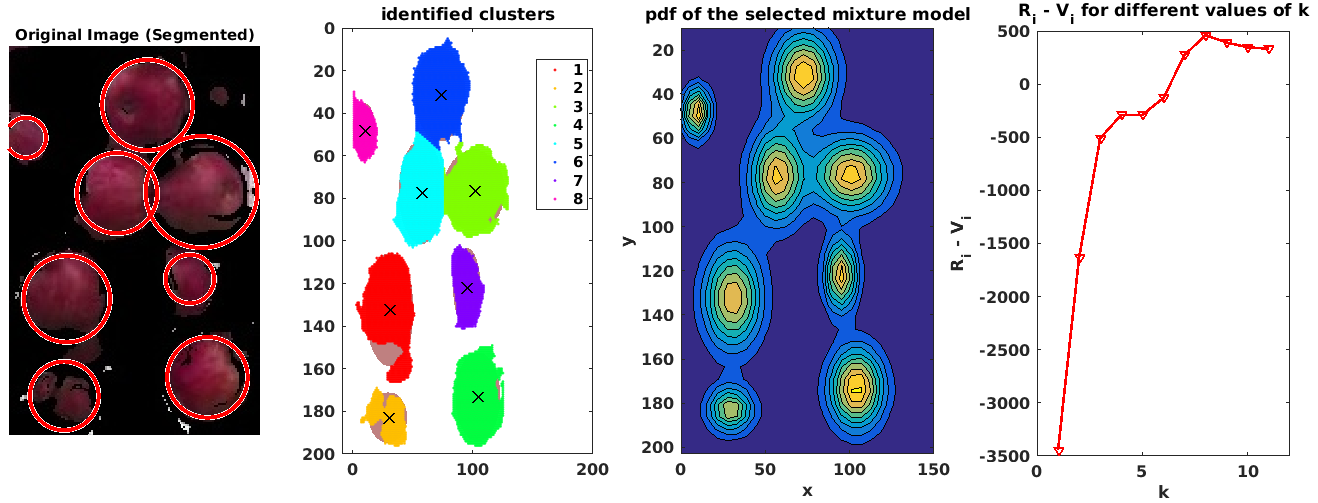
\includegraphics[width=\textwidth]{figures/counting/applejournalcountreal.png}           
        
   %\caption{An example from the GMM counting method.
   \label{fig:gmmex}  
  \caption[Fruit counting on real data using unsupervised clustering.]{A sample output from GMM on real data.}
   \label{fig:grpcongmm}
\end{figure}    

\subsection{Greedy Circle Fitting Method}\label{subsec:greedycount}
The GMM method uses a global fitting criterion to segment the fruit. In this section, we present a greedy approach that achieves reasonable performance efficiently. In the case of images containing single fruit, with a rough knowledge of fruit radius in terms of pixels, we can create Gaussian kernels of different sizes within the known bounds, convolve the entire image with them and find the maximum response location to find the center of the fruit. This concept can be extended in the case of images containing more fruit. The first fruit is chosen as the fruit with the maximum kernel response. Likewise, the second one can be computed by choosing another fruit, which combined with the previously chosen one maximizes the total response of both. In this method, the order in which the fruit is selected defines an occlusion hierarchy. The response of the combination of multiple Gaussian kernels is computed using this hierarchy. Fig.~\ref{fig:groupex}(\subref{fig:greedy}) shows a detected apples on an input image from the greedy method. It is unable to detect the partially visible apple. Fig.~\ref{fig:groupex}(\subref{fig:gmcomp}) shows the output of GMM method on the same input. It successfully finds the apple missed by the greedy method.


\section{Experimental Results}\label{experiments}
In this section, we rigorously study the performance of the counting method.  This study can be separated into three parts. First, we evaluate the performance of the GMM-based counting with the greedy circle fitting method on independent datasets.   Afterward, we study the performance of the GMM-based method on datasets presented in Chapter~\ref{chapter:detection}. Finally, we compare the GMM-based method to a superior deep learning approach developed by  H{\"a}ni et al.~\cite{hani_jfr_counting}. 

\subsection{Comparison with Greedy Circle Fitting}
We evaluated the performance of our clustering-based counting algorithm with the greedy circle fitting method on four different datasets obtained from different platforms. The first two datasets were obtained from hand-held cameras, the third dataset from a camera mounted on a ground vehicle and the fourth dataset from a camera mounted on a flying UAV. Fig.~\ref{fig:datasets} shows sample images from all four datasets. It is notable that for these datasets the images were segmented using hard color thresholds~\cite{techreportroy}.

\begin{figure}[!hbpt]
        \centering
        \begin{subfigure}[b]{.20\textwidth}
            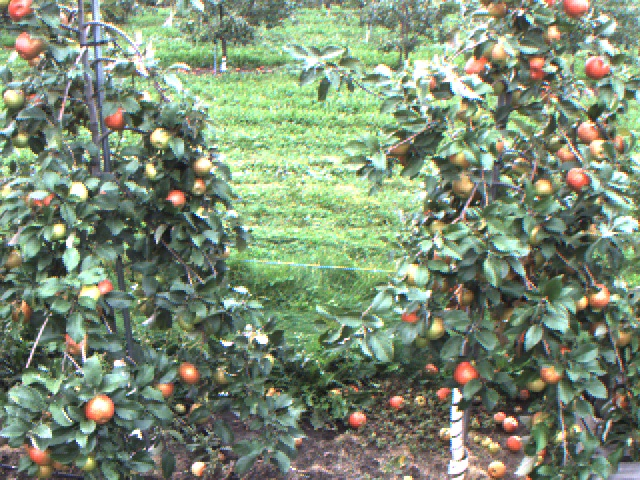
\includegraphics[width =\textwidth]{figures/counting/dataset1.jpg}           
       \end{subfigure}\quad \begin{subfigure}[b]{.20\textwidth}
            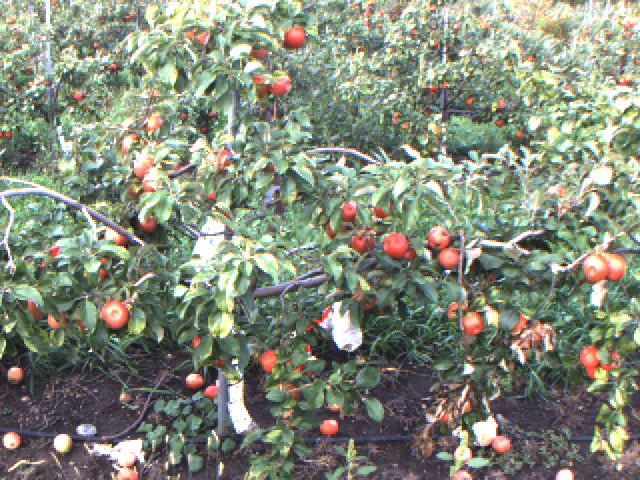
\includegraphics[width = \textwidth]{figures/counting//dataset2.jpg}           
        \end{subfigure}\quad \begin{subfigure}[b]{.22\textwidth}
            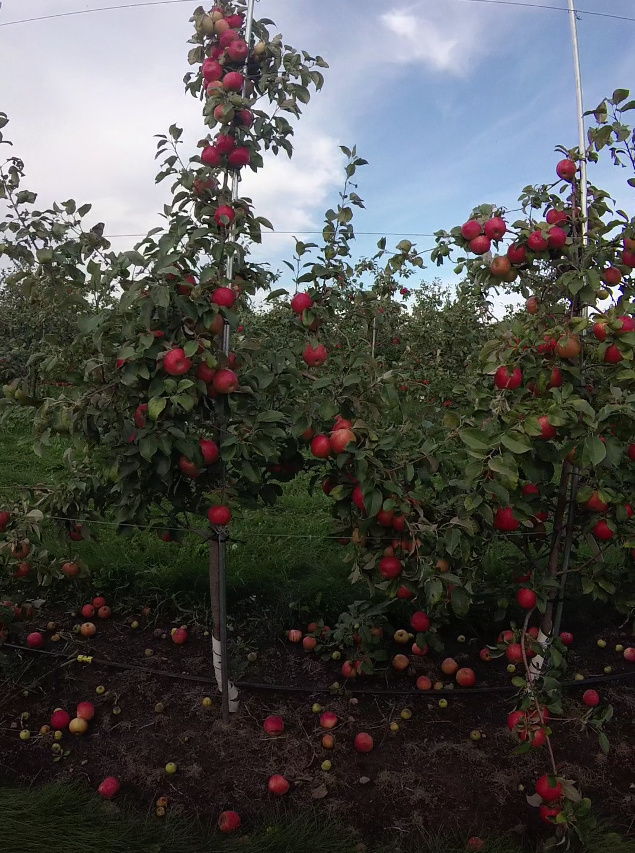
\includegraphics[width = \textwidth]{figures/counting/dataset31.jpg}           
       \end{subfigure}\quad \begin{subfigure}[b]{.20\textwidth}
            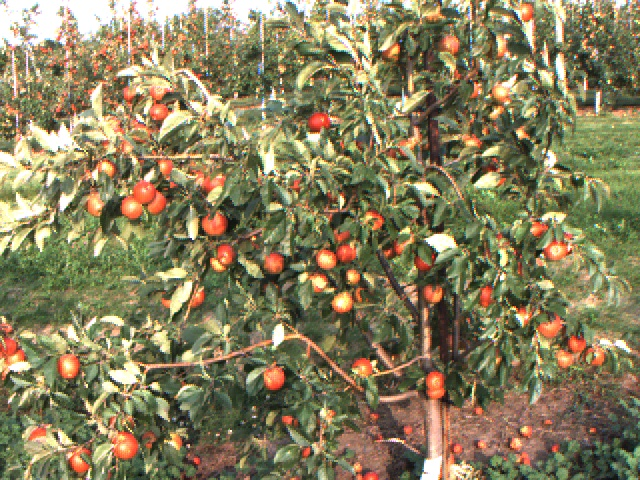
\includegraphics[width = \textwidth]{figures/counting/dataset4.jpg}           
       \end{subfigure}
   \caption[Sample images from test datasets for comparison with greedy circle fitting.]{Sample images from test datasets for comparison with greedy circle fitting. The two images on the left are obtained from hand-held cameras. The third image from left is obtained from a camera mounted on a ground vehicle and the rightmost image is obtained from a camera mounted on a UAV.}
   \label{fig:datasets}
\end{figure}    



We first evaluate the GMM method with the segmented apple clusters from Dataset~3. (Fig.~\ref{fig:groupex}(\subref{fig:sapple1}),~\ref{fig:groupex}(\subref{fig:capple1}) ). We used $442$ such images for this purpose, all of which were hand-counted. We identified clusters of different sizes (Fig.\ref{fig:oanalysis}(\subref{fig:segdata})) and evaluated the performance of our algorithm in terms of accuracy, overcounting and undercounting per cluster size (Fig.~\ref{fig:oanalysis}(\subref{fig:clusterAnlysis})). The overall accuracy for the entire dataset is $91.30\%$. For clusters containing six or more apples, the percentage of undercounting goes up to $33.33\%$. The number of instances of such large-sized clusters was very low to make any strong inference about the performance of the algorithm. For single apples, we found $10\%$ overcounting. This problem can be attributed to occlusion and specularities which make the algorithm think that there are two apples instead of one.

\begin{figure*}[tbp]
        \centering
        \begin{subfigure}[b]{.3\textwidth}
        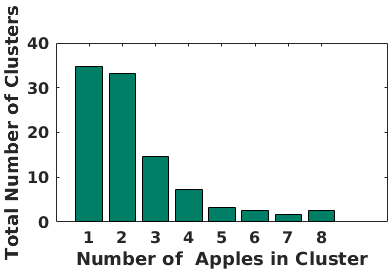
\includegraphics[width=\textwidth]{figures/counting/countAnalysisData31.png}
        \caption{The distribution of different size clusters}
             \label{fig:segdata}
        \end{subfigure}\quad \begin{subfigure}[b]{.65\textwidth}
                 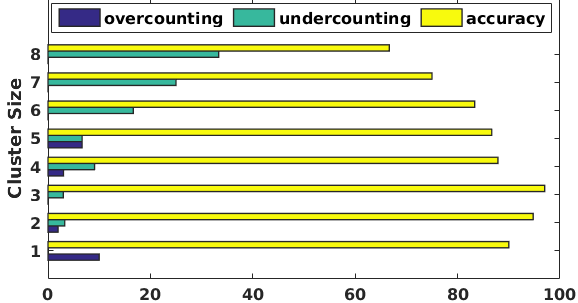
\includegraphics[width=\textwidth]{figures/counting/clusterAnalysis31.png} 
                 \caption{Performance of the GMM based counting method across different cluster size}
                     \label{fig:clusterAnlysis}   
        \end{subfigure}\\ \begin{subfigure}[b]{.9\textwidth}
                     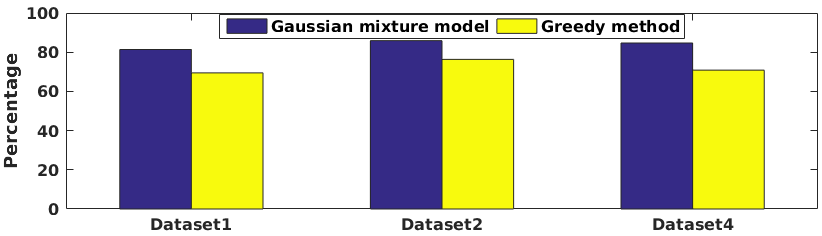
\includegraphics[width = \textwidth]{figures/counting/redgreen31.png}   
                     \caption{Performance of the counting pipeline for Dataset 1,2 and 4}
                     \label{fig:grossres}
        \end{subfigure}
   \caption[Performance comparison of unsupervised clustering based fruit counting to greedy circle fitting.]{Performance comparison of unsupervised clustering based fruit counting to greedy circle fitting.}
   \label{fig:oanalysis}
\end{figure*}    

%\subsection{Gross Results}
%The gross results across the entire dataset is one of the most crucial end product for an automatic yield estimation system. 

Next, we evaluate the total performance of our counting pipeline using the Dataset 1, 2 and 4. Dataset 1 contains a mixture of red and green apples. The total number of images in this dataset is $464$. It covers a block in an orchard row containing six trees. Dataset 2  primarily contains red apples. The total number of images in this dataset is $964$. It covers a full row in an orchard. Dataset4 was collected using a UAV. It contains $655$ images and covers six trees. The total number of hand-counted apples from the images in the datasets is $258$ and $952$, and $673$ respectively. The accuracy of the GMM counting method for the first and second and fourth dataset is $81.3492\%$, $85.87\%$ and $84.72\%$. The drop in accuracy for the first dataset is mainly attributed to our segmentation method~\cite{techreportroy} where many green apples were not detected. Fig.~\ref{fig:oanalysis}(\subref{fig:grossres}) shows a bar chart of the accuracy of our counting methods. We show the accuracy of the greedy method for comparison. For the greedy counting method, the accuracy drops down to $69.44\%$ for the first dataset and $76.34\%$ for the second dataset. This drop is expected as the greedy method uses a hard threshold for grouping apple pixels. It fails when the scale of the image varies a lot or apples are only partially visible. Fig.~\ref{fig:grossres} shows a bar chart of the accuracy of our counting method for the first two datasets.



%\begin{figure}[tbp]
%        \centering
%        
%            \includegraphics[width=.5\textwidth]{newfigs/countRedGreen}           
%        
%   \caption{Gross result from handheld datasets.}
%   \label{fig:grossres}
%\end{figure}    
%
\subsection{Performance Evaluation on Datasets from Chapter~\ref{chapter:detection}}\label{subsec:count_res} for Scalability
In this section, we quantify the performance of our counting method on the test datasets mentioned in Chapter~\ref{chapter:detection}. These datasets are bigger than the independent datasets used for comparison with the greedy circle fitting method in the previous section. The same datasets were also used to evaluate the overall yield estimation performance of the full system in Chapter~\ref{chapter:map_yield}. Therefore, it is crucial to examine the performance of the counting algorithm on these datasets. 

To evaluate the per-frame counting algorithm, we took all the segmented images from seven videos collected from the four datasets. Afterward, we performed a connected component analysis on them, randomly selected $5000$ components and marked each one with the perceived count from a human point of view. These counts are then compared to the counts obtained from the algorithm. At this stage, we want the segmented images to be accurate and consequently, we use the \supemph{user-supervised} model presented in Chapter~\ref{chapter:detection} for detection.
\begin{figure*}[!hbpt]
        \centering
        \begin{subfigure}[b]{\textwidth}\begin{subfigure}[b]{.55\textwidth}
                 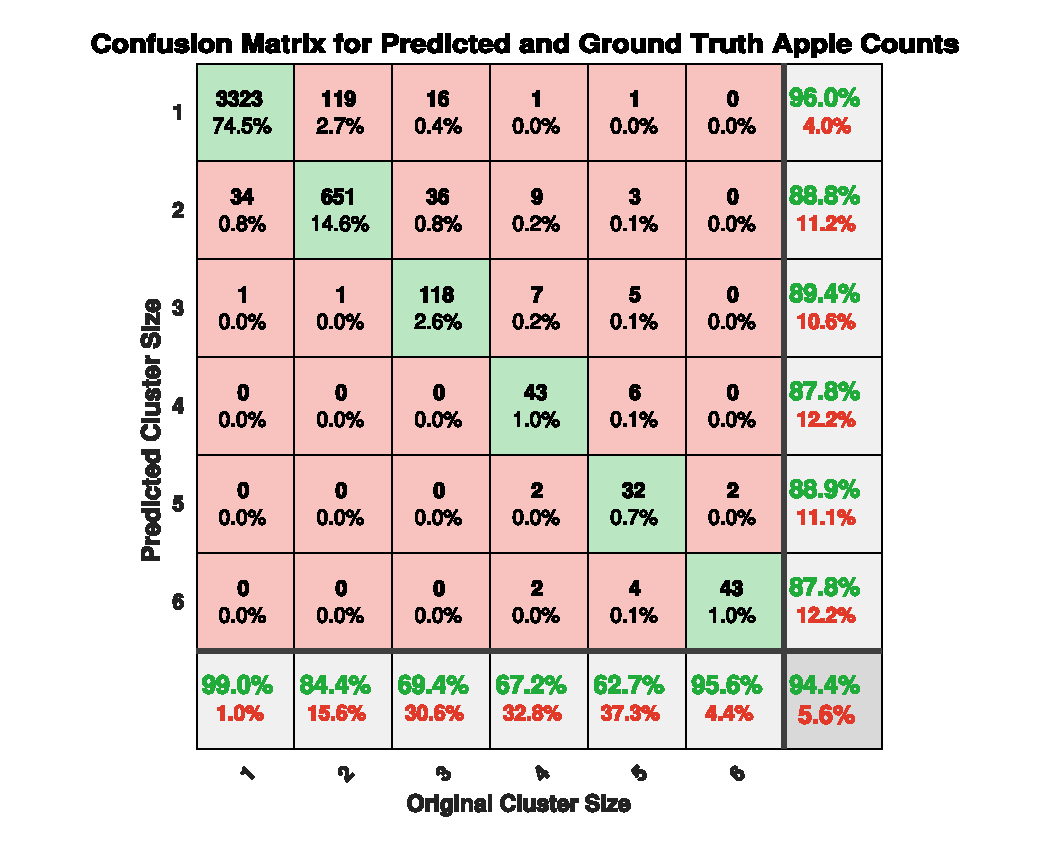
\includegraphics[width=\textwidth]{figures/counting/confusionmat.pdf}
                 \caption{Confusion matrix for the per-frame counting method.}
                     \label{fig:confusionmat}   
        \end{subfigure}\quad \begin{subfigure}[b]{.40\textwidth}
                         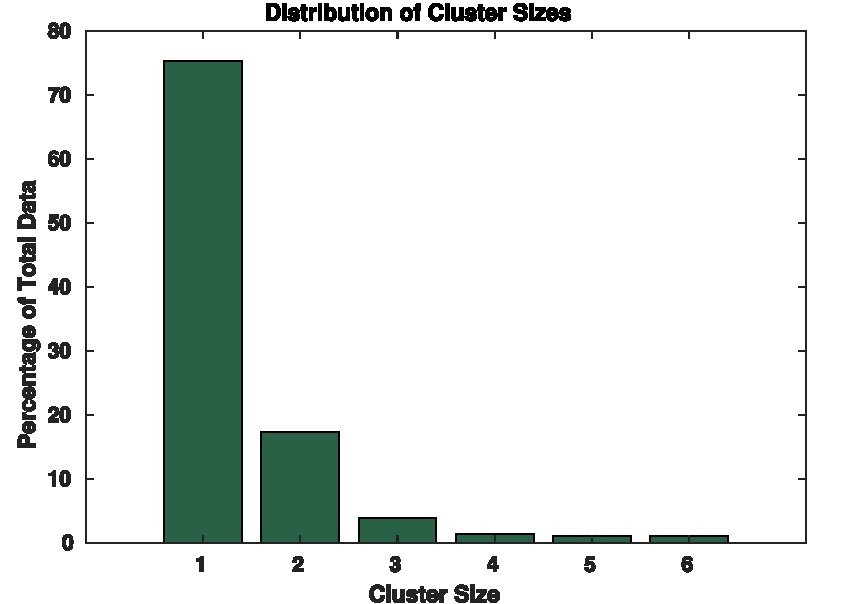
\includegraphics[width=\textwidth]{figures/counting/ClusterDist.pdf}
                 \caption{Distribution of cluster sizes.}
                     \label{fig:clusterDist}   
        \end{subfigure}
        \end{subfigure}\\ \begin{subfigure}[b]{\textwidth}
        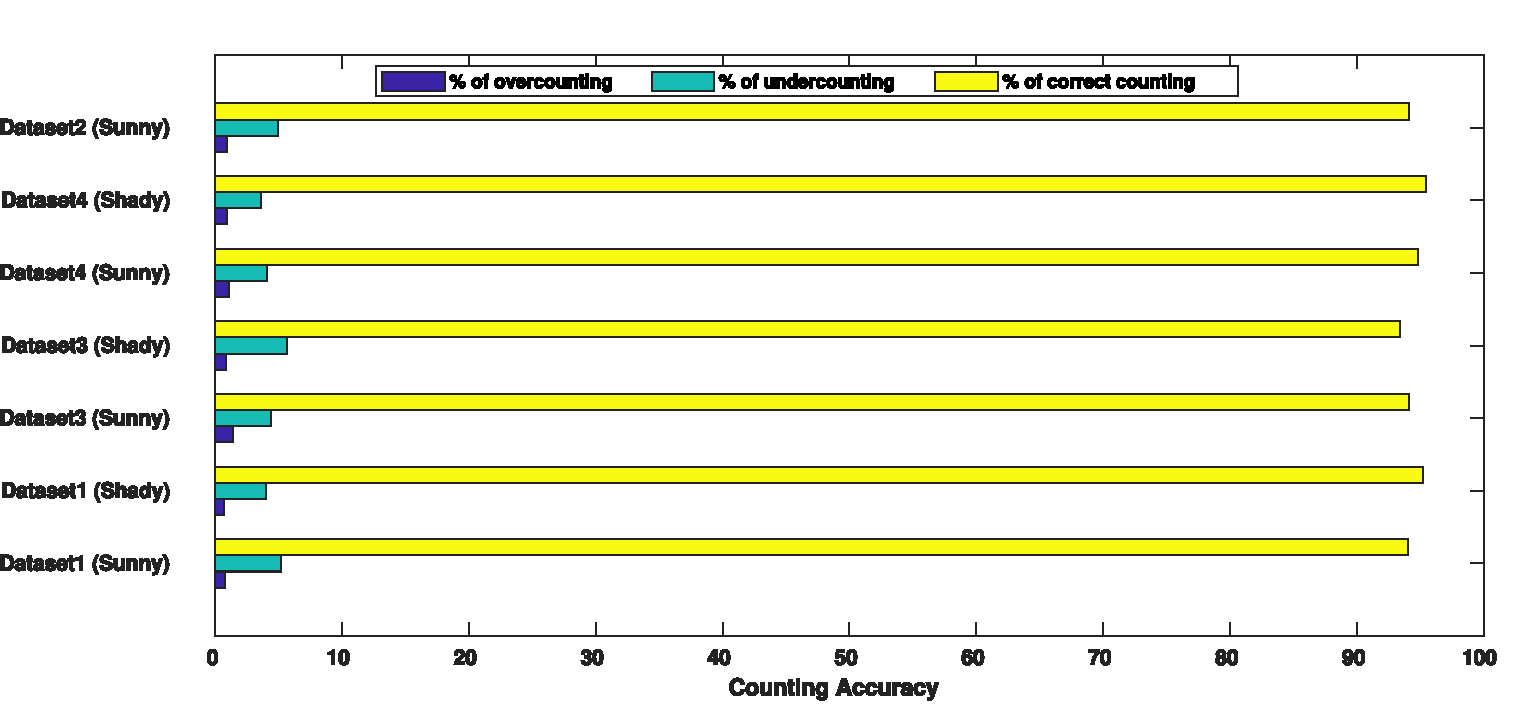
\includegraphics[width=\textwidth]{figures/counting/datasetcount_.pdf} 
        \caption[Per-frame accuracy of the unsupervised counting method]{Accuracy of the per-frame counting method across different videos collected from Dataset1-Dataset4.}
             \label{fig:countdatasets}
        \end{subfigure}
   \caption[Evaluation of the unsupervised fruit counting method on Datasets from Chapter~\ref{chapter:detection}.]{Evaluating the performance of the per-frame counting algorithm on Datasets from Chapter~\ref{chapter:detection}- confusion matrix (left), distribution of cluster sizes (middle) and performance across different datasets (right). The right-bottom cell in the confusion matrix (figure on left) shows that the overall accuracy of our method is $94.4\%$. The rightmost column (Rows $1-6$) shows the precision per cluster size and the bottom row (Columns $1-6$) shows recall per cluster size. From the figure in the middle, we find that single apple clusters are dominating the data ($75.31\%$). The figure on right shows how our counting accuracy varied from $94.01\% - 95.38\%$ across different videos.}
   \label{fig:analysis}
\end{figure*}    

To understand the effect of cluster size on the counting algorithms, we look at the confusion matrix plots in Fig.~\ref{fig:confusionmat}. In these plots, the rows correspond to the predicted number of apples (Output) and the columns correspond to the true apple count (Target). The diagonal cells correspond to observations that are correctly classified. The off-diagonal cells correspond to incorrectly classified observations. Both the number of observations and the percentage of the total number of observations are shown in each cell. The column on the far right of the plot shows the overall precision. The row at the bottom of the plot shows the overall recall. The cell in the bottom right of the plot shows the overall accuracy.

Essentially, we have three key insights from this experiment. First, it is evident from the confusion matrix (Fig.~\ref{fig:analysis}(\subref{fig:confusionmat})), that recall drops with increasing cluster size (varies from $62.7\% - 99\%$) but precision stays over $87\%$ for any cluster size (varies from $87.8\% - 96\%$). Second, for a large portion of the data - single apples ($75.31\%$ of entire data (Fig.~\ref{fig:analysis}(\subref{fig:clusterDist}))); the precision and recall of our algorithm are $96\%$ and $99\%$ respectively. Consequently, the overall accuracy of our method is high ($94.4\%$) (shown in the right-bottom cell in the confusion matrix). Third, low recall rates for larger clusters do not affect the overall performance. 

Next, we quantify the effect of lighting conditions (sunny, shady, cloudy, etc.) on the counting method. We computed the accuracy of the per-frame counting method across all the collected videos (which were collected in different lighting conditions). Our counting accuracy varied from $94.01\% - 95.38\%$. Undercounting percentage varies from $3.62\%- 5.67\%$ and overcounting varies from $.74\% - 1.1\%$. These results are presented in Fig.~\ref{fig:analysis}(\subref{fig:countdatasets}).


\subsection{Comparison with the Deep Learning Approach from H{\"a}ni et. al.~\cite{hani_jfr_counting}}\label{subsec:count_result}
In 2018, H{\"a}ni et al.~\cite{hani_jfr_counting} formulated the accurate counting of clustered fruit as a classification problem with a finite number of classes (maximum cluster size is limited to six) per Region of Interest (RoI). They solved this multi-class classification problem using a state-of-the-art deep residual network ResNet50~\cite{he_deep_2015}.  This method takes the detected ROI's, that are likely to contain fruit, as inputs. The network can receive input from a variety of detection algorithms. For example, any of the methods described in Chapter~\ref{chapter:detection} would produce acceptable image patches. This approach is superior to the clustering method in the sense that it does not require the detection masks and it can reject false positives. 
\begin{figure*}[!hbpt]
    \centering
    \def\svgwidth{0.95\textwidth}
     \def\svgwidth{\textwidth}
    \import{figures/counting/}{cnn_count_schematic.pdf_tex}\label{fig:cnn}
    \caption[Counting using classification network.]{Schematic drawing of counting using classification network. (a) Input image with detected regions of interest; (b) Extracted regions; (c) ResNet50 for classification of image patches; (d) Patches are classified into 7 counts.}
    \label{fig:cnnpipeline}
\end{figure*}

Here, we compare the performance of the GMM-based counting approach to the CNN-based methods.  The train and test datasets for the CNN were collected from the same location as in Chapter~\ref{chapter:detection}.

\textbf{Training Sets: }The cluster counting network was trained using two datasets. One of these datasets contains green, and one contains red apples. They were acquired from same tree rows as datasets 5 and 6 described in Chapter~\ref{chapter:detection} (see Fig.~\ref{fig:train}) in 2015. Both datasets were obtained from the sunny side of the tree row. From these two datasets, image patches were extracted using the user-supervised detection method described in Section~\ref{sec:segmentation}. In total, $13000$ image patches were annotated manually. Additionally, $4500$ patches were extracted at random that do not contain apples. To balance the class distribution the training dataset was up-sampled using random data augmentation (horizontal flipping, rotations of $\pm 5^\circ$ and Gaussian smoothing), to a total of $\sim65,000$ image patches.

\textbf{Validation Sets: }To supervise the network during training, we used an $80/20 \%$ split of the available data for training/validation.

\textbf{Test Sets: } For testing we used four datasets. The final datasets are composed of a total of $2874$ images. See Table~\ref{tab:datacount} for dataset details.

\begin{table}[ht!]
    \begin{center}
        \caption{Overview of the apple counting test datasets}
        \label{tab:datacount}
        \begin{tabular}{|c|c|c|}
            \hline
            \textbf{Dataset} & \specialcell{\textbf{Number of} \\ \textbf{image patches}}  & \textbf{Characteristics} \\
            \hline
            1 & 956 & \specialcell{Red apples, \\ contains patches from the sunny and shady side of the tree row}\\
            \hline
            2 & 628 & \specialcell{Yellow and orange apples, \\ contains patches from the sunny side of the tree row} \\
            \hline
            3 & 587 & \specialcell{Green apples, \\ contains patches from the sunny and shady side of the tree row} \\
            \hline
            4 & 703 & \specialcell{Red apples, \\ contains patches from the sunny side of the tree row \\ acquired from larger distance (apples appear at lower resolution)} \\
            \hline
        \end{tabular}
    \end{center}
\end{table}

Using these datasets, we evaluated the counting performance of the GMM and CNN based methods. Table~\ref{tab:1} shows the counting accuracy.

\begin{table}[h!]
    \begin{center}
        \caption{Image Patch Counting Results}
        \label{tab:1}
        \begin{tabular}{|c|c|c|c|c|}
            \hline
            \textbf{Approach} & \textbf{Test Set 1} & \textbf{Test Set 2} & \textbf{Test Set 3} & \textbf{Test Set 4}\\
            \hline
            GMM & 88.0 \% & 81.8 \% & 77.2 \% & 76.1 \% \\
            \hline
            ResNet50 & \textbf{88.8} \% & \textbf{92.68 \%} & \textbf{95.1 \%} & \textbf{88.5 \%}\\
            \hline
        \end{tabular}
    \end{center}
\end{table}

The ResNet50 network outperforms the GMM model on all of the test sets. On test set 3, the CNN outperforms the GMM by almost $11\%$. On test sets 2 and 4 it outperforms the GMM by $18\%$ and $12\%$ respectively. These results show that the neural network generalizes between datasets even under varying illumination conditions and among data sets with different colors.


The confusion matrices in Fig.~\ref{fig:confmat} show that the GMM is precise in predicting a single apple. For all other categories, the performance of the method drops considerably. In contrast, the neural network's performance drops slowly in cases of higher fruit counts. Additionally, we see that the deep network can reject false positive detections in $87\%$ of the cases. Comparably, the GMM does so in only $43\%$ of the cases. The distribution of apples in these test datasets though is highly skewed towards one single apple. We observed this phenomenon throughout our experiments, as the majority of clusters returned by the detection method are in the range $\lbrack 0, 4 \rbrack$. 

\begin{figure}[!htbp]
    \centering
    \begin{subfigure}[b]{0.46\textwidth}
    \centering
    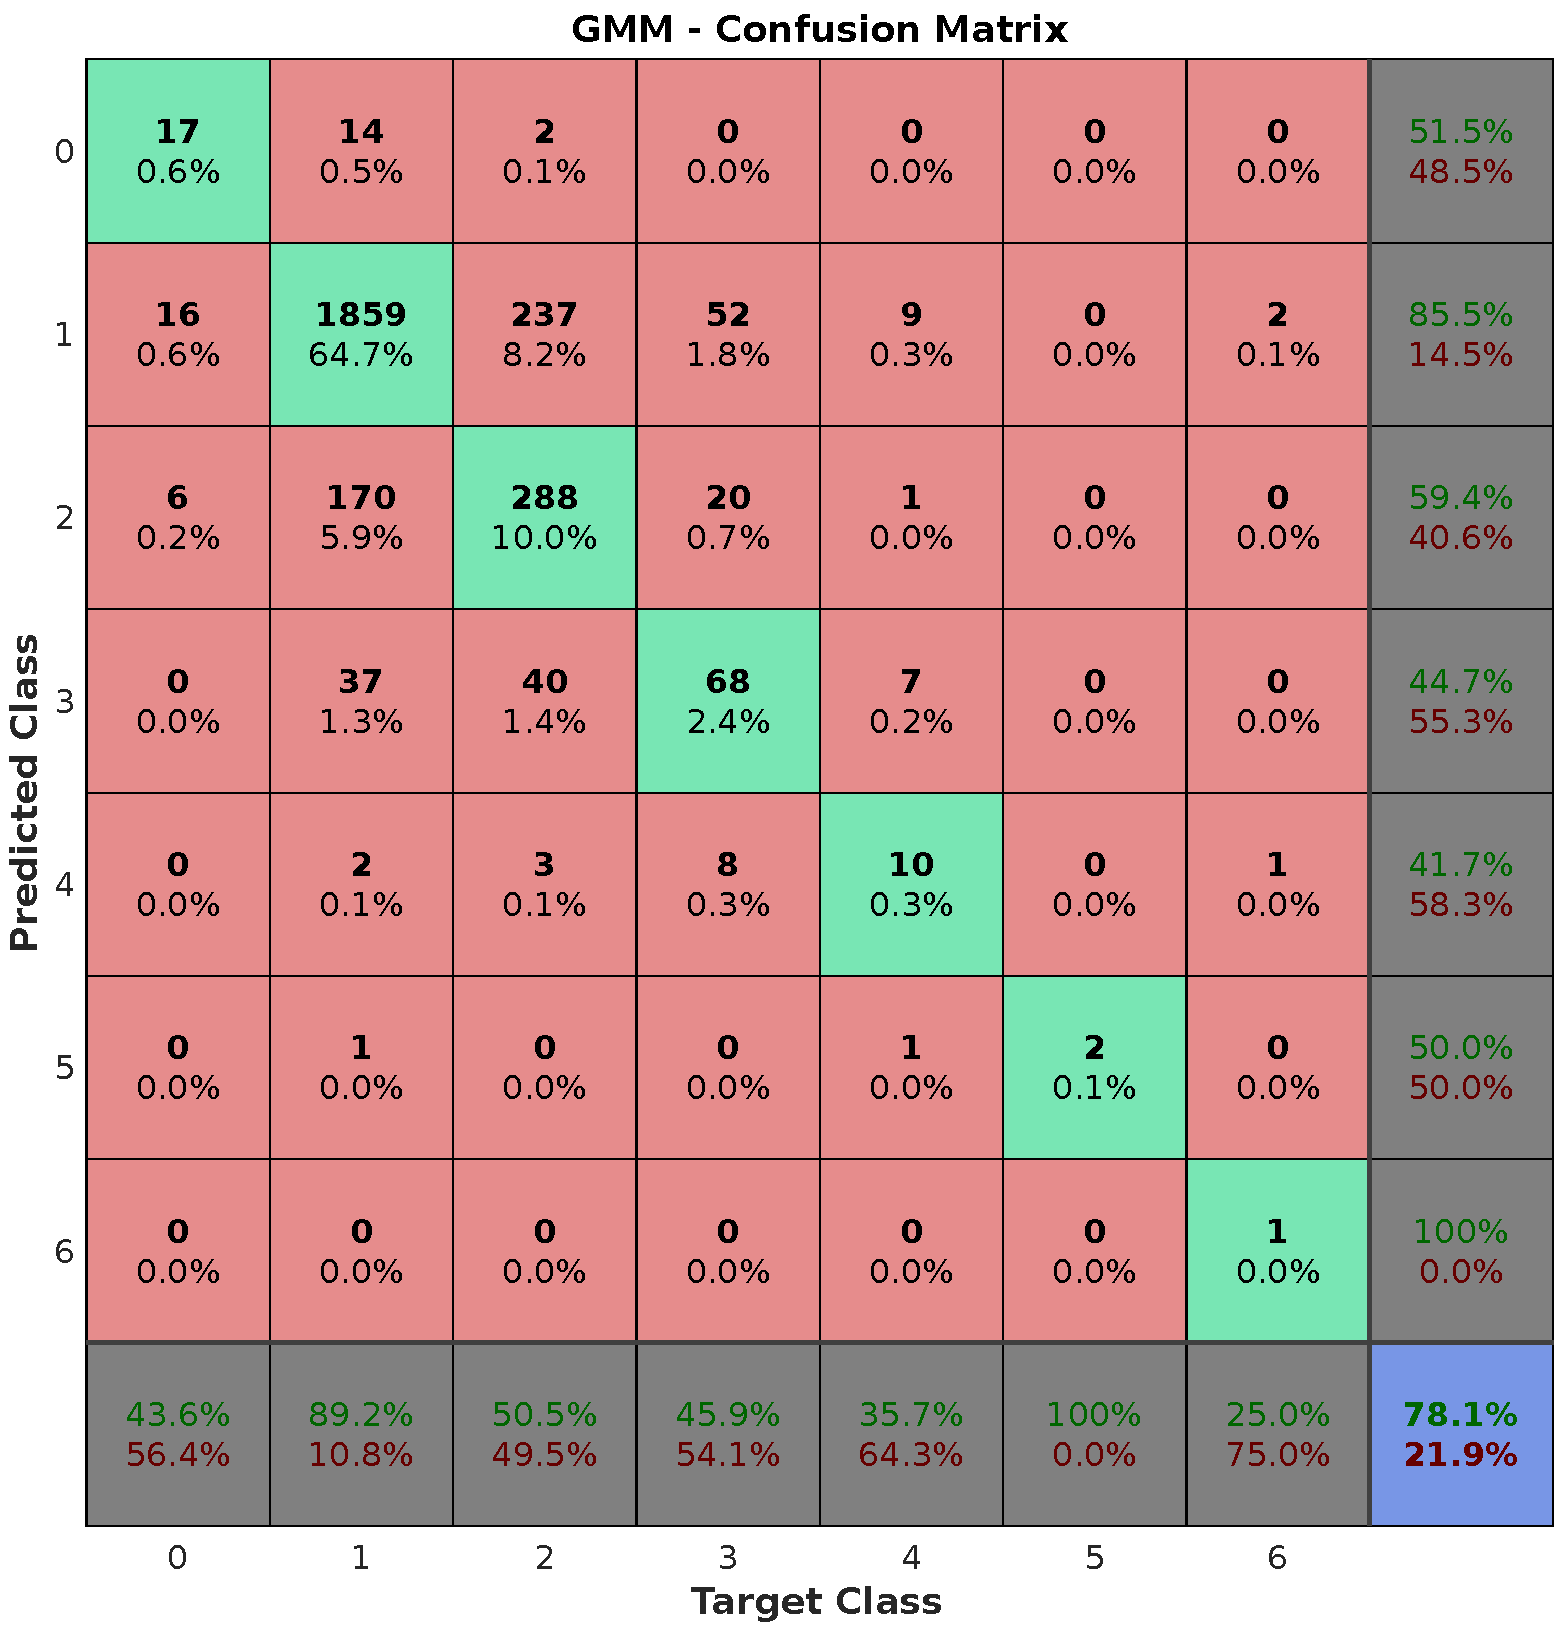
\includegraphics[width=\textwidth]{figures/counting/gmm_confmat.pdf}%
    \caption{GMM confusion matrix}
    \end{subfigure}
    \quad \begin{subfigure}[b]{0.46\textwidth}
    \centering
    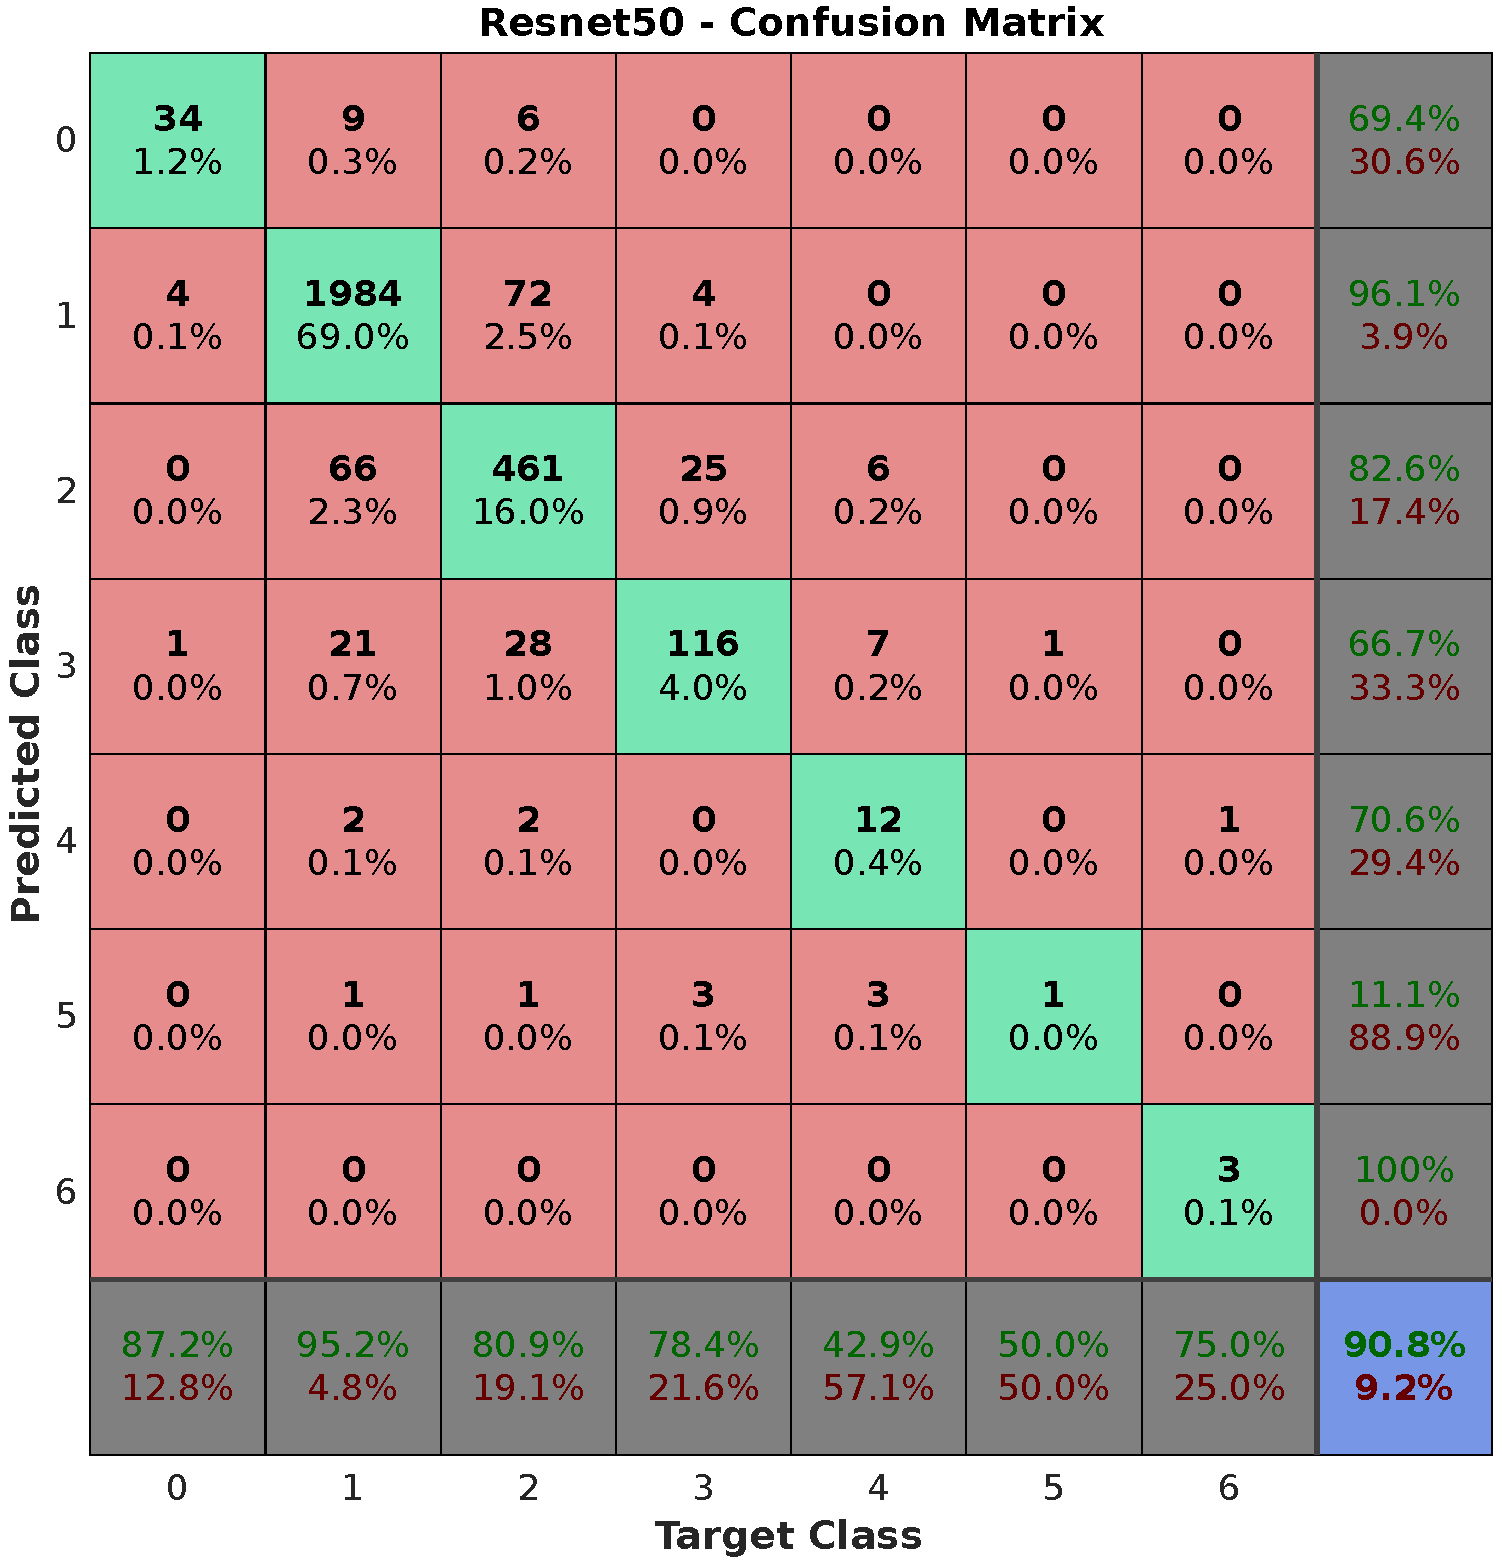
\includegraphics[width=\textwidth]{figures/counting/resnet_confmat.pdf}%
    \caption{ResNet50 confusion matrix}
    \end{subfigure}
    \caption[Comparison of counting performance with H{\"a}ni et al.~\cite{hani_jfr_counting}]{Confusion matrices over all four test datasets}
    \label{fig:confmat}
\end{figure}



\section{Experimental Insights and Conclusion}\label{sec:conc}
In this chapter, we presented a method for counting fruit from segmented input images. While the results are encouraging, there is still room for improvement. The algorithm fails to predict the correct number of fruit when there is too much overlap and boundaries among different fruit are not detectable. To get a better insight into this problem, we show a synthetic input where the algorithm fails (Fig. ~\ref{fig:wrong}). Here, the predicted number of components by the algorithm is five but the actual number is six. A closer look at the solution from the EM algorithm for $k = 6$ shows that actually, EM failed to find out the correct location and pixel radius of fruit which resulted in large coverage penalty and low circularity. These types of problems are present in natural conditions too. One such observation is shown in  Fig.~\ref{fig:grpfail}. For these types of scenarios, it is hard to predict the correct number of fruit from a single view. 

\begin{figure}[!htbp]

        \centering        
            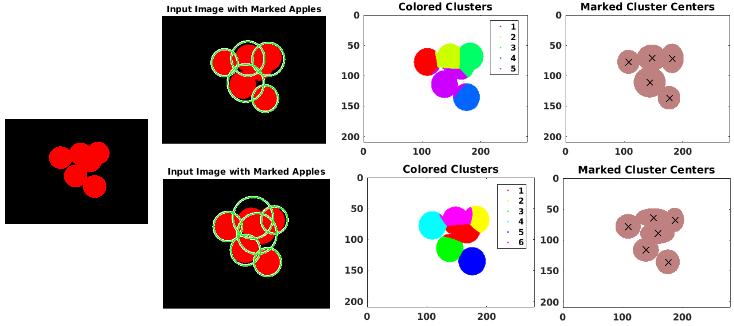
\includegraphics[width = .8\textwidth]{figures/counting/wrong.png}           
        
   \caption[A failure case for the unsupervised clustering based counting on synthetic data.]{A synthetic input where the algorithm fails to compute $k$ correctly. If we look closely at the solution found by EM for the correct $k$, we find that EM failed to find the correct location which resulted in large coverage penalty and low circularity. }
   \label{fig:wrong}   
\end{figure}    

\begin{figure}[!htbp]
    \centering
            \centering
            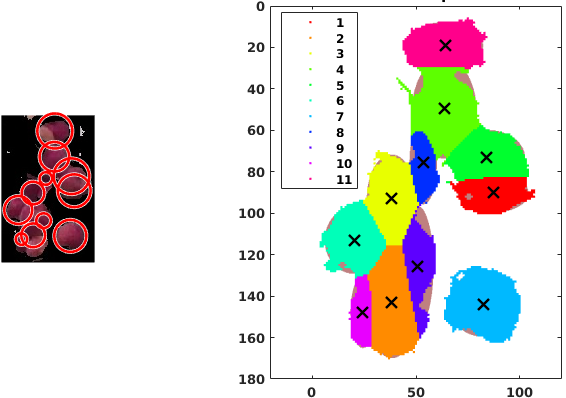
\includegraphics[width = .8\textwidth]{figures/counting/emfail3.png}
       
        \caption[A failure case for the unsupervised clustering based counting on real data.]{A failure case in real data. Here, EM failed to find out the correct location and pixel radius of fruit which resulted in large coverage penalty and low circularity}
   \label{fig:grpfail}

\end{figure}

The deep learning-based counting approach proposed by  H{\"a}ni et al.~\cite{hani_jfr_counting}, although achieving overall $90.5\%$ accuracy, suffers from similar problems when fruits are partially visible. A natural way to resolve these ambiguities is to use active vision (look at the cluster from another viewpoint). We present such a method in Chapter~\ref{chapter:active_counting}. In the next chapter, we move our focus to more geometric computer vision problems. We start with a method to recover the underlying scene geometry for tracking the fruits.